\documentclass[conference,10pt]{IEEEtran}
\IEEEoverridecommandlockouts
\usepackage[T1]{fontenc}
\usepackage{amsmath,amssymb}
\usepackage{graphicx}
\usepackage{booktabs}
\usepackage{multirow}
\usepackage{xcolor}
\usepackage{algorithm}
\usepackage{algpseudocode}
\usepackage{tikz}
\usetikzlibrary{positioning,arrows.meta,fit,backgrounds}
\usepackage[hidelinks]{hyperref}
\usepackage{cite}

\definecolor{prop}{HTML}{2a78d6}
\definecolor{ink2}{HTML}{52514e}
\newcommand{\ours}{\textsc{CloudForensiX}}

\begin{document}

\title{\ours: Implementing and Evaluating a Forensic-Ready Monitoring and Incident-Response Framework Derived from the Cloud Forensics Survey of Manral~\textit{et al.}}

\author{
\IEEEauthorblockN{Aditya Sharma, Atithi Jaiman, Ashish Singh}
\IEEEauthorblockA{Course: Cloud and SRE Security --- Monitoring and Incident Response\\
Department of Computer Science and Engineering\\
Code: \url{https://github.com/4uashish2628/cloudsre}}
}

\maketitle

\begin{abstract}
Manral \textit{et al.}'s systematic survey of cloud forensics (ACM CSUR, 2019) organises a decade of research into incident-, provider-, consumer- and resource-driven solutions. It closes with a set of investigation guidelines: live and remote analysis, forensic log aggregation and correlation, the CSP as a forensic contributor, privacy and evidence isolation, and trusted computing. It also identifies a gap in forensic \emph{metrics}. The survey reports that most reviewed proposals lack an implementation or an evaluation. This paper turns those guidelines into a working, end-to-end system and measures it. \ours{} combines five components:
(i) FRSL, a tamper-evident log that couples a hash chain with Merkle-sealed epochs, anchored \emph{Proofs of Past Logs} MAC-ed by the tenant, and Bloom filters;
(ii) time-normalised aggregation of five heterogeneous cloud log formats;
(iii) a hybrid detector that contextualises rules with a learnt behaviour profile;
(iv) an entity-graph correlator with multi-hop timeline reconstruction; and
(v) tenant-isolated, Merkle-sealed evidence packages with a hash-linked chain-of-custody ledger.
The evaluation uses a seeded multi-tenant IaaS simulator with 20 ground-truth attack campaigns per run and benign look-alikes, over five seeds and eight experiments.
FRSL detected 100\% of insider tampering, including attacks in which the insider recomputes every stored hash; the plain hash chain detected none of those. FRSL ingests 7.2$\times$ faster than a proof-of-work blockchain log, and an inclusion proof verifies a single record about 5,300$\times$ faster than a full audit.
The hybrid detector cut false alerts by 67\% relative to rules alone (14.6 vs.\ 44.2 per day) while still detecting all campaigns, with a mean time to detect of 83\,s.
Entity-graph correlation achieved an ARI of 0.9996. Reconstruction raised evidence recall from 34\% (alerted events only) to 100\%.
Inventory-based time normalisation was essential: without it, recall for SSH lateral movement fell to 63\%.
Evidence isolation removed all 51 foreign-tenant identifiers per incident while retaining every attack record.
The whole pipeline sustains about 52k records/s on a laptop.
\end{abstract}

\begin{IEEEkeywords}
cloud forensics, incident response, forensic readiness, secure logging, log correlation, event reconstruction, multi-tenancy, SRE security
\end{IEEEkeywords}

%=====================================================================
\section{Introduction}
Incidents in the cloud are investigated under constraints that conventional digital forensics never had to face. The physical location of the evidence is unknown. Resources are virtualised and shared between tenants. Logs are spread across the tenant, the service owner and the cloud service provider (CSP), each with its own format and clock. The investigator must also trust the provider that operates the infrastructure~\cite{manral2019,pichan2015,nist8006}. For site reliability engineering (SRE) and security operations this is not abstract: the same telemetry pipeline that drives alerting must, after an incident, be able to produce evidence that is complete, correctly ordered and demonstrably unaltered.

Manral \textit{et al.}~\cite{manral2019} survey cloud forensic research from 2009 to 2019. They propose a taxonomy (incident-driven, provider-driven, consumer-driven and resource-driven forensics), map the forensic artifacts held by each stakeholder (their Table~14), and conclude with five investigation guidelines. Their comparative tables repeatedly note that individual proposals \emph{``lack implementation and model evaluation''}. They also observe that no metrics exist for comparing forensic solutions.

This paper addresses that gap for the \emph{Monitoring and Incident Response} track of a Cloud and SRE Security course. We treat the survey's guidelines as a specification, implement them as one coherent system, and evaluate each design decision against the baselines the survey discusses. Our contributions are:
\begin{enumerate}
\item \textbf{A requirements analysis.} We derive six requirements (R1--R6) from the survey's guidelines and taxonomy, and use them to position the surveyed solutions (Table~\ref{tab:req}).
\item \textbf{\ours{}, an open-source framework} that realises all six requirements in one pipeline: continuous tamper-evident collection (FRSL), heterogeneous aggregation with time normalisation, hybrid live detection, entity-graph correlation and reconstruction, tenant isolation, and chain of custody. It is about 2,300 lines of Python with 28 unit tests.
\item \textbf{FRSL}, a secure-logging scheme. It addresses the weaknesses the survey lists for SecLaaS and BlockSLaaS, namely a malicious CSP and computational overhead, by anchoring tenant-MAC-ed Merkle epochs outside CSP control.
\item \textbf{A reproducible evaluation methodology}: a seeded multi-tenant IaaS simulator that emits raw logs in five real-world formats with ground truth, and a forensic metric suite (detection, reconstruction, integrity, privacy and acquisition metrics) answering the gap the survey identifies in its Sec.~7.2.
\item \textbf{Eight experiments} quantifying the trade-offs, including two negative results: the unsealed-window vulnerability, and the naive-timestamp ablation.
\end{enumerate}

%=====================================================================
\section{Background and Related Work}
\label{sec:related}
\subsection{The survey's taxonomy}
Manral \textit{et al.}~\cite{manral2019} classify solutions as follows:
\emph{incident-driven} solutions are either continuous (forensic readiness) or post-incident;
\emph{provider-driven} solutions are log-based or agent-based;
\emph{consumer-driven} solutions use physical acquisition or the management plane;
\emph{resource-driven} solutions target VM, storage or network forensics.
\ours{} is mainly incident-driven, continuous and provider-assisted. It also contains a consumer-driven element, since logs are anchored with tenant keys, and a resource-driven one, since it correlates VM, storage and network artifacts.

\subsection{Secure logging}
Zawoad \textit{et al.}'s SecLaaS~\cite{zawoad2016} stores logs with a \emph{Proof of Past Log} (PPL) and uses Bloom filters for fast integrity checks. CLASS~\cite{ahsan2018} adds asymmetric encryption and Rabin fingerprints. BlockSLaaS~\cite{rane2019} writes encrypted entries to a blockchain, and Wang \textit{et al.}~\cite{wang2019} use a third-party auditor with Merkle-structured tags on a blockchain. The survey criticises these schemes for not considering a malicious CSP, for not validating logs before verification, and for their overhead (Table~4 of~\cite{manral2019}). Hash chains and Merkle trees for tamper-evident logs go back to Schneier and Kelsey~\cite{schneier1999} and Crosby and Wallach~\cite{crosby2009}. FRSL combines these primitives with the threat model the survey calls for.

\subsection{Forensic readiness and central logging}
Trenwith and Venter~\cite{trenwith2013} argue for central logging with authenticated, time-stamped transport. Marty~\cite{marty2011} gives logging guidelines for SaaS. Kebande and Venter's CFREAS~\cite{kebande2015} proposes MapReduce analysis of readiness data, but without a prototype. The ``forensic-by-design'' principle~\cite{abrahman2016} asks for forensic capability to be built into cloud systems from the outset.

\subsection{Management-plane acquisition}
FROST~\cite{dykstra2013} adds forensic APIs to OpenStack for acquiring virtual disks, API logs and firewall logs, but it requires trust in the CSP. Alex and Kishore's forensic monitoring plane~\cite{alex2017} centralises evidence outside the cloud, at the cost of introducing a single point of failure.

\subsection{Event reconstruction}
CLOSER~\cite{raju2017} applies the Leader-Follower (LF) aggregation algorithm to cloud service logs, and a later framework~\cite{raju2018} reconstructs VM artifact timelines. Section~8.2.2 of the survey states that log correlation is crucial but under-studied. We use LF as the state-of-the-art baseline for correlation.

\subsection{Metrics}
Cohen~\cite{cohen2011} discusses evidence-level metrics. The survey (Sec.~7.2) notes the absence of metrics for comparing cloud forensic solutions and suggests analysis time, effort, alert latency and false positives. These suggestions shape our metric suite.

\begin{table}[t]
\centering
\caption{Requirements derived from the survey and coverage by surveyed solutions (\checkmark{} = addressed, $\circ$ = partially, -- = not).}
\label{tab:req}
\footnotesize
\setlength{\tabcolsep}{3pt}
\resizebox{\columnwidth}{!}{\begin{tabular}{p{3.4cm}cccccc}
\toprule
Requirement (survey section) & \rotatebox{70}{SecLaaS\cite{zawoad2016}} & \rotatebox{70}{BlockSLaaS\cite{rane2019}} & \rotatebox{70}{FROST\cite{dykstra2013}} & \rotatebox{70}{FMP\cite{alex2017}} & \rotatebox{70}{CLOSER\cite{raju2017}} & \rotatebox{70}{\textbf{Ours}} \\
\midrule
R1 continuous, tamper-evident collection robust to a malicious CSP (3.1, 4.1, 8.2.3) & $\circ$ & $\circ$ & -- & $\circ$ & -- & \checkmark \\
R2 heterogeneous aggregation and time normalisation (8.2.2, 7.1.2) & -- & -- & -- & -- & $\circ$ & \checkmark \\
R3 live detection: quick alerts, few false positives (8.2.1, 7.2) & -- & -- & -- & $\circ$ & -- & \checkmark \\
R4 correlation and event reconstruction (4.1, 8.2.2) & -- & -- & -- & -- & \checkmark & \checkmark \\
R5 privacy and evidence isolation (8.2.4) & -- & -- & $\circ$ & -- & -- & \checkmark \\
R6 integrity, chain of custody, measurable outcome (5, 7.2, 8.2.5) & $\circ$ & $\circ$ & $\circ$ & $\circ$ & -- & \checkmark \\
Prototype and evaluation reported & \checkmark & $\circ$ & \checkmark & -- & \checkmark & \checkmark \\
\bottomrule
\end{tabular}}
\end{table}

%=====================================================================
\section{System and Threat Model}
\label{sec:model}
\paragraph*{Stakeholders} Following Sec.~8.1 of the survey, we distinguish the cloud \emph{end-user} (U), the \emph{service owner} or tenant (O), and the \emph{CSP} (P). The CSP comprises the hypervisor, the cloud management software, storage management and network management. Table~14 of the survey records which of these parties each artifact depends on.

\paragraph*{Environment} A multi-tenant IaaS region hosts $T$ tenants. Each tenant has users, VMs and object-storage buckets, and the VMs share hypervisor nodes. Five artifact sources are in scope: control-plane API logs (CloudTrail-like; O/P), VPC flow logs (O/P), guest-OS syslog (O/P), hypervisor logs (P), and storage access logs (P).

\paragraph*{Adversaries}
(A1) An \emph{external attacker} who compromises credentials or hosts and carries out one of five campaign types (Sec.~\ref{sec:setup}).
(A2) A \emph{malicious CSP insider}, as stressed in Sec.~8.2.3 of the survey, with full read/write access to the log store. A2 can modify, delete, insert, reorder or truncate records and recompute every stored hash, but cannot forge the tenant's anchor MAC key or rewrite anchors that have already been published.
(A3) An \emph{honest-but-curious co-tenant or investigator}, whose access to another tenant's data would violate privacy (Sec.~8.2.4).

\paragraph*{Goals} When an incident occurs, the investigator should receive a complete, correctly ordered, integrity-verifiable and tenant-isolated evidence set. It should arrive quickly, with as little dependence on the CSP as possible.

%=====================================================================
\section{The \ours{} Framework}
\label{sec:design}

\begin{figure*}[t]
\centering
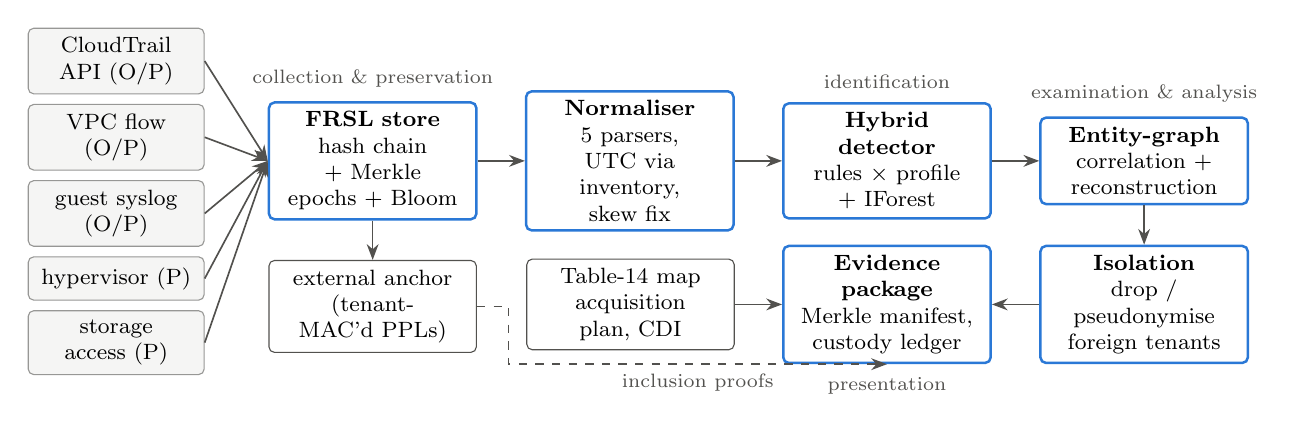
\begin{tikzpicture}[font=\footnotesize, node distance=4mm and 6mm,
  box/.style={draw=ink2, rounded corners=2pt, align=center, minimum height=9mm, text width=24mm, fill=white},
  pbox/.style={box, draw=prop, line width=0.9pt},
  src/.style={draw=ink2!60, rounded corners=2pt, align=center, text width=20mm, minimum height=5.5mm, fill=ink2!6},
  arr/.style={-{Stealth[length=2mm]}, ink2, line width=0.6pt}]
\node[src] (ct) {CloudTrail API (O/P)};
\node[src, below=1.2mm of ct] (fl) {VPC flow (O/P)};
\node[src, below=1.2mm of fl] (sy) {guest syslog (O/P)};
\node[src, below=1.2mm of sy] (hv) {hypervisor (P)};
\node[src, below=1.2mm of hv] (s3) {storage access (P)};
\node[pbox, right=8mm of fl, yshift=-3mm] (frsl) {\textbf{FRSL store}\\hash chain + Merkle\\epochs + Bloom};
\node[box, below=5mm of frsl, text width=24mm] (anc) {external anchor\\(tenant-MAC'd PPLs)};
\node[pbox, right=of frsl] (norm) {\textbf{Normaliser}\\5 parsers, UTC via\\inventory, skew fix};
\node[pbox, right=of norm] (det) {\textbf{Hybrid detector}\\rules $\times$ profile\\+ IForest};
\node[pbox, right=of det] (cor) {\textbf{Entity-graph}\\correlation +\\reconstruction};
\node[pbox, below=5mm of cor] (iso) {\textbf{Isolation}\\drop / pseudonymise\\foreign tenants};
\node[pbox, left=of iso] (pkg) {\textbf{Evidence package}\\Merkle manifest,\\custody ledger};
\node[box, left=of pkg] (art) {Table-14 map\\acquisition plan, CDI};
\foreach \s in {ct,fl,sy,hv,s3} \draw[arr] (\s.east) -- (frsl.west);
\draw[arr] (frsl) -- (anc);
\draw[arr] (frsl) -- (norm);
\draw[arr] (norm) -- (det);
\draw[arr] (det) -- (cor);
\draw[arr] (cor) -- (iso);
\draw[arr] (iso) -- (pkg);
\draw[arr] (art) -- (pkg);
\draw[arr, dashed] (anc.east) -- ++(4mm,0) |- (pkg.south) node[pos=0.75, below, font=\scriptsize, ink2]{inclusion proofs};
\node[font=\scriptsize, ink2, above=0.5mm of frsl] {collection \& preservation};
\node[font=\scriptsize, ink2, above=0.5mm of det] {identification};
\node[font=\scriptsize, ink2, above=0.5mm of cor] {examination \& analysis};
\node[font=\scriptsize, ink2, below=0.5mm of pkg] {presentation};
\end{tikzpicture}
\caption{Architecture of \ours{}. Proposed components are outlined in blue. Stage labels follow the five-stage investigation process used by the survey (its Fig.~1).}
\label{fig:arch}
\end{figure*}

Fig.~\ref{fig:arch} shows the pipeline. Its stages follow the survey's five-stage investigation process. Unlike hypervisor-level approaches such as ForenVisor~\cite{qi2017}, it requires no modification of the CSP's virtualisation layer.

\subsection{FRSL: Forensic-Ready Secure Log (R1, R6)}
\label{sec:frsl}
Each raw record $m_i$ is appended as entry $e_i=(i, m_i, h_{i-1}, h_i)$, where
\begin{equation}
h_i = H\big(i \,\|\, h_{i-1} \,\|\, m_i\big),\qquad h_{-1}=0^{256},
\end{equation}
and $H$ is SHA-256. Every $B$ entries (an \emph{epoch} $k$), FRSL builds a Merkle tree~\cite{merkle1987} over $h_{s_k},\dots,h_{s_k+B-1}$, with domain-separated leaf and node hashes, giving a root $r_k$. It then emits a Proof of Past Log
\begin{align}
\mathrm{PPL}_k &= \big(k, s_k, n_k, r_k, h_{s_k+n_k-1}, H(\mathrm{PPL}_{k-1})\big),\\
\tau_k &= \mathrm{MAC}_{K_T}(\mathrm{PPL}_k),
\end{align}
The key $K_T$ belongs to the tenant or its auditor, never the CSP. $(\mathrm{PPL}_k,\tau_k)$ is published to an append-only anchor such as a tenant bucket, a transparency log or a consortium ledger. A Bloom filter~\cite{bloom1970} over $H(m_i)$, sized for a $10^{-3}$ false-positive rate, accompanies each PPL. It lets an investigator test whether a record existed without downloading the epoch, which is the SecLaaS use case~\cite{zawoad2016}.

\emph{Audit} recomputes the chain, checks each $\tau_k$ and the PPL linkage, and recomputes each epoch's root and tail. \emph{Single-record verification} checks one $e_i$ against $\tau_k$ using a Merkle inclusion proof of $\lceil\log_2 B\rceil$ hashes.

\emph{Security argument.} Suppose A2 modifies, inserts, deletes or reorders an entry inside a sealed epoch. That changes either the leaf set or the count of the epoch, and therefore $r_k$ or $n_k$. Matching the anchor would then require a SHA-256 collision or a forged MAC. Recomputing the chain does not help, because the anchor fixes $r_k$, $n_k$ and the chain tail. Truncation removes epochs, or entries within an epoch, whose PPLs are already anchored. The \emph{only} undetectable window is the unsealed tail, which is at most $B-1$ entries. We measure this window explicitly in E3.

\subsection{Aggregation and time normalisation (R2)}
Five parsers map raw lines to one event schema: time, tenant, action, principal, source and destination IP, port, bytes, resource, created identity, host, region and outcome. Each event also gets a set of \emph{forensic entities} (principal, external IP, created identity and host).

The parsers must resolve three time problems. RFC~3164 syslog has no year or time zone, so we take the host zone from the tenant's asset inventory and the year from the case. Hypervisor nodes log in their own zone with drifting clocks, so we subtract the drift recorded by an NTP audit. Attacker-launched VMs are absent from the inventory, so the normaliser \emph{learns} IP-to-instance mappings online from \texttt{RunInstances} responses.

\subsection{Hybrid live detection (R3)}
\textbf{Rules.} R1--R6 are Sigma-style correlation rules for: brute force followed by success (console or SSH), administrator-policy attachment or a key created for another user, audit tampering (\texttt{StopLogging}, \texttt{DeleteTrail}, \texttt{auditd stop}, log shredding), mining-pool traffic or bursts of instance launches in an unusual region, bulk object collection, and large external egress.

\textbf{Anomaly model.} An Isolation Forest~\cite{liu2008} is trained on 12-dimensional per-entity, 10-minute behaviour vectors from a clean baseline period (the first 6\,h of each run).

\textbf{Hybrid (proposed).} During the baseline period we learn a profile $P$ of (principal, source IP) and (IP, action) pairs. Bulk-collection, egress and brute-force alerts whose evidence lies entirely inside $P$ are suppressed, as are IAM or launch-burst alerts that originate from the corporate egress and stay in the home region. Alerts outside the profile are kept, and anomalies above a stricter threshold (the 99.9th training percentile plus a margin) are added. This implements the survey's call for ``quick alerts with minimum false positives'' while staying explainable: every suppression records its reason.

\subsection{Entity-graph correlation and reconstruction (R4)}
Algorithm~\ref{alg:eg} groups alerted events into incidents using union-find. Events from the same alert are always merged. Two events of the same tenant are merged if they share an entity within that entity's horizon. \emph{Strong} entities (external IPs, identities created during the incident) link across 4\,h. \emph{Weak} entities (an existing principal or host, which unrelated campaigns may also hit) link only across 30\,min.

Reconstruction then performs a 2-hop entity pivot over \emph{all} events in $[t_{\text{start}}-30\,\text{min},\, t_{\text{end}}+4\,\text{h}]$. Host pivots pull in only security-relevant host events: SSH, sudo, audit, VM start, saturated-CPU heartbeats, and flows to port 22 or to external non-HTTPS peers. IPs used by more than three identities (for example a corporate NAT) are pruned as infrastructure supernodes.

\begin{algorithm}[t]
\caption{Entity-graph correlation}
\label{alg:eg}
\footnotesize
\begin{algorithmic}[1]
\Require alerted events $E$ (time-sorted), alerts $A$, horizons $\Delta_s,\Delta_w$
\State $\textsc{uf}\gets$ union-find over $E$;\; $\textit{last}\gets\emptyset$
\For{$a\in A$} \textsc{union} all events of $a$ \EndFor
\For{$e\in E$}
  \For{$x\in \textit{ent}(e)$}
     \State $\Delta\gets\Delta_s$ \textbf{if} $x\in\textit{strong}(e)$ \textbf{else} $\Delta_w$
     \If{$(e.\textit{tenant},x)\in\textit{last}$ \textbf{and} $e.t-\textit{last}[\cdot].t\le\Delta$}
        \State \textsc{union}$(e, \textit{last}[\cdot].e)$
     \EndIf
     \State $\textit{last}[(e.\textit{tenant},x)]\gets(e.t,e)$
  \EndFor
\EndFor
\State \Return connected components as incidents
\end{algorithmic}
\end{algorithm}

\subsection{Evidence isolation (R5)}
For tenant $T$, events attributed to other tenants are dropped. Shared records, such as hypervisor node statistics that list every co-resident VM, are kept only if they concern $T$. Foreign identifiers in them (VM names, tenant ids, account ids and private IPs) are replaced by $\mathrm{HMAC}_{K_{\text{escrow}}}$ pseudonyms, which a court-authorised key holder can re-identify.

\subsection{Chain of custody and the artifact map (R6)}
Each incident becomes an evidence package containing:
\begin{itemize}
\item the reconstructed timeline;
\item the isolated raw records;
\item the alerts;
\item an acquisition plan derived from the survey's Table~14;
\item FRSL inclusion proofs for the records;
\item a Markdown report.
\end{itemize}
Every artifact's SHA-256 enters a Merkle manifest. A custody ledger records each action (open, acquire, seal, transfer, verify) as a hash-linked entry, MAC-ed by the acting party. The \emph{CSP Dependency Index} (CDI) of an incident is the fraction of its required sources that are obtainable only through the CSP.

\subsection{Forensic metrics}
We report the following metrics:
\begin{itemize}
\item event-level precision, recall, F1 and false-positive rate (FPR);
\item alert precision and false alerts per day;
\item campaign detection rate and mean time to detect (MTTD);
\item clustering ARI, V-measure and fragmentation (incidents per campaign);
\item timeline recall and precision, and pairwise ordering accuracy;
\item tamper-detection rate per attack class;
\item foreign-identifier leakage;
\item CDI and evidence acquisition time (EAT).
\end{itemize}

%=====================================================================
\section{Implementation and Experimental Setup}
\label{sec:setup}
\ours{} is implemented in Python 3.14 (NumPy, pandas, scikit-learn) as eight modules, together with a CLI and 28 \texttt{pytest} tests. All experiments run with one command (\texttt{make experiments}, about 65\,s) on an Apple M5 laptop with 16\,GB of RAM.

\paragraph*{Why a simulator} The survey notes that researchers cannot instrument commercial CSP back-ends (Sec.~1 of~\cite{manral2019}), and public cloud forensic datasets with ground-truth campaign labels across stakeholders are scarce. We therefore built a deterministic simulator that emits \emph{raw text} in the five formats of Table~\ref{tab:data}, with hidden ground truth (true UTC time, label, campaign and kill-chain step) that is used only for scoring.

\paragraph*{Benign activity} Benign traffic follows a diurnal profile. It includes deliberate \emph{confounders} that resemble attacks: forgotten passwords, travelling users who fail to log in 5--7 times from a never-seen IP, nightly backups with bulk downloads and large egress, a disaster-recovery drill from a new site, legitimate administrator grants (including some \texttt{AdministratorAccess}), GPU batch launches, and Internet SSH scanners.

\paragraph*{Attacks} Twenty campaigns per 24-hour run, four of each type, start at random times between hours 6 and 21 in random tenants, so they overlap in time:
\begin{enumerate}
\item \emph{credential\_exfil}: console brute force, bucket discovery, 80--200 object downloads, then access-key persistence.
\item \emph{priv\_esc}: IAM reconnaissance with access-denied errors, a new user with \texttt{AdministratorAccess}, and a new key.
\item \emph{cryptomining}: 5--10 GPU instances launched in an unusual region, with 1--3\,h of mining-pool traffic.
\item \emph{ssh\_lateral}: SSH brute force, a dropper, an internal port-22 sweep, then pivoting to two further VMs.
\item \emph{anti\_forensics}: a hijacked administrator stops CloudTrail, deletes flow logs, stops \texttt{auditd} and shreds \texttt{auth.log}.
\end{enumerate}
Results are averaged over seeds 1--5; $\pm$ values are standard deviations.

\begin{table}[t]
\centering
\caption{Simulated artifact sources (seed 1, 4 tenants, 24\,h; 36.9k records).}
\label{tab:data}
\footnotesize
\setlength{\tabcolsep}{3pt}
\begin{tabular}{llcl}
\toprule
Source & Format modelled on & Dep. & Time quirk \\
\midrule
cloudtrail & AWS CloudTrail JSON & O/P & UTC \\
vpcflow & VPC Flow Logs v2 & O/P & epoch seconds \\
syslog & RFC 3164 guest OS & O/P & local zone, no year \\
hypervisor & libvirt host log & P & node zone + drift (to $\pm$45\,s) \\
s3access & S3 server access log & P & UTC offset \\
\bottomrule
\end{tabular}
\end{table}

%=====================================================================
\section{Results}
\label{sec:results}

\subsection*{E1--E2: Cost of tamper-evident collection}
Fig.~\ref{fig:e1} and Table~\ref{tab:log} compare the five logging schemes.

FRSL ingests about \textbf{321k entries/s} on a single core. That is 7.2$\times$ faster than a proof-of-work blockchain log with only 12-bit difficulty (44k/s), and about 6$\times$ slower than an unanchored hash chain. Its storage overhead (52.5\%) is dominated by the per-entry chain fields (72\,B) for these short records. PPLs and Bloom filters add only 1.4 percentage points.

A full audit of 50k entries takes 43\,ms. A single-record Merkle proof is 10 hashes (320\,B) and verifies in \textbf{8\,$\mu$s}, about 5,300$\times$ faster than an audit. This makes per-record verification practical for evidence packages. The measured Bloom-filter false-positive rates match their design targets (Table~\ref{tab:log}).

\begin{figure}[t]
\centering
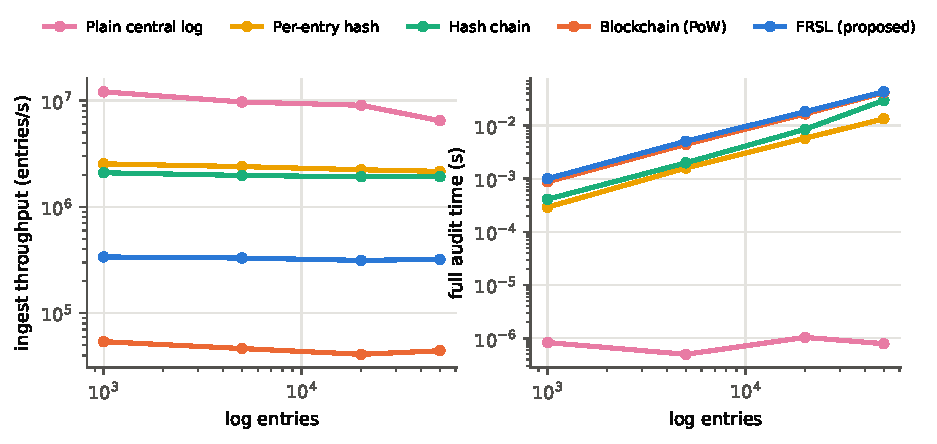
\includegraphics[width=\columnwidth]{figures/e1_throughput_verify.pdf}
\caption{E1: ingest throughput (left) and full-audit time (right) against log size. The plain log has no audit.}
\label{fig:e1}
\end{figure}

\begin{table}[t]
\centering
\caption{E1--E3 at 50k entries. Tamper column: share of the 10 attack settings detected.}
\label{tab:log}
\footnotesize
\setlength{\tabcolsep}{3.5pt}
\begin{tabular}{lrrrr}
\toprule
Scheme & entries/s & overhead & audit (ms) & tamper det. \\
\midrule
Plain central log & 6.46M & 0\% & -- & 0\% \\
Per-entry hash & 2.16M & 22.7\% & 13 & 20\% \\
Hash chain & 1.92M & 51.1\% & 30 & 40\% \\
Blockchain (PoW) & 44.2k & 24.4\% & 42 & 100\% \\
\textbf{FRSL (proposed)} & \textbf{321k} & 52.5\% & 43 & \textbf{100\%} \\
\midrule
\multicolumn{5}{l}{Bloom filter (10k items), target FP $10^{-2}/10^{-3}/10^{-4}$}\\
\multicolumn{5}{l}{\quad measured FP $0.997\%/0.083\%/0.009\%$}\\
\bottomrule
\end{tabular}
\end{table}

\subsection*{E3: Tamper detection against a malicious CSP}
Fig.~\ref{fig:e3} shows detection rates over 100 trials per cell on 2,000-entry logs.

Per-entry hashes miss deletions, reordering and truncation. A hash chain detects every edit, but \emph{none} once the insider recomputes the chain, which is exactly the malicious-CSP case the survey flags as unaddressed. Only externally anchored schemes, FRSL and the blockchain, detect all ten settings.

\emph{Window of vulnerability (negative result).} If the insider strikes before the open epoch is sealed, truncation of the unsealed tail goes unnoticed. The detection rate for random-point truncation falls from 100\% at $B{=}64$ (15 unsealed entries) to 89\% at $B{=}256$, 51\% at $B{=}1024$, and 0\% when nothing has been sealed. Operators should therefore seal on a timer (for example every few seconds) as well as on size. A forensic-readiness SLA should state the seal interval.

\begin{figure}[t]
\centering
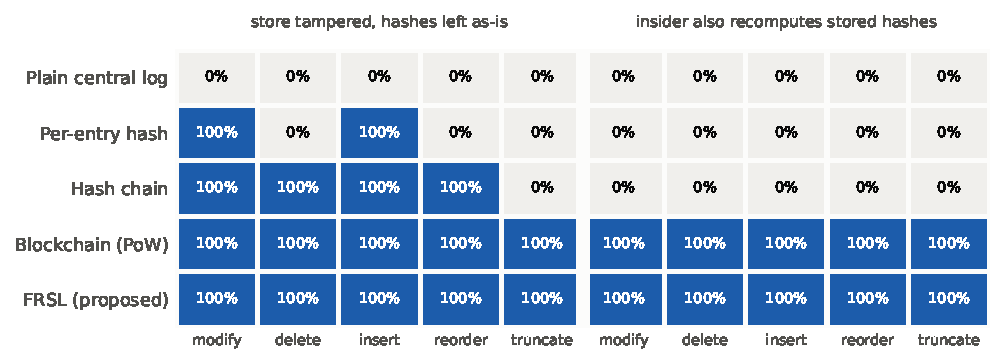
\includegraphics[width=\columnwidth]{figures/e3_tamper_heatmap.pdf}
\caption{E3: tamper-detection rate per scheme and insider attack (100 trials each).}
\label{fig:e3}
\end{figure}

\subsection*{E4: Live detection}
Table~\ref{tab:det} and Fig.~\ref{fig:e4} compare the detectors.

The rules detect every campaign but raise 44 false alerts a day, because the confounders trigger them. The Isolation Forest alone is unsuitable as a trigger: only 10\% of its alerts are true, and it finds 26\% of campaigns. It catches bulk exfiltration but misses low-volume steps such as \texttt{StopLogging} or a single policy attachment.

The hybrid keeps the rules' 100\% campaign detection and 83\,s MTTD. It cuts false alerts by \textbf{67\%} (14.6/day), raises event precision from 0.49 to 0.78, and lowers the FPR to 0.95\%. The remaining false positives are confounders that are genuinely novel: travelling users and the disaster-recovery drill from a new site. Event-level recall stays at about 0.39 because detectors flag only the \emph{triggering} events. Recovering the rest is the job of reconstruction (E5).

\begin{table}[t]
\centering
\caption{E4: detection quality (mean $\pm$ std over 5 seeds, 20 campaigns each).}
\label{tab:det}
\footnotesize
\setlength{\tabcolsep}{2.4pt}
\resizebox{\columnwidth}{!}{\begin{tabular}{lcccccc}
\toprule
Detector & Prec. & F1 & FPR & Alert prec. & False/day & Campaigns \\
\midrule
Rules & .49$\pm$.04 & .44$\pm$.02 & 3.5\% & .72$\pm$.02 & 44.2$\pm$5.9 & 100\% \\
IForest & .42$\pm$.03 & .44$\pm$.02 & 5.5\% & .10$\pm$.01 & 78.8$\pm$9.1 & 26\% \\
\textbf{Hybrid} & \textbf{.78$\pm$.08} & \textbf{.52$\pm$.03} & \textbf{0.95\%} & \textbf{.89$\pm$.03} & \textbf{14.6$\pm$5.0} & \textbf{100\%} \\
\bottomrule
\end{tabular}}
\end{table}

\begin{figure}[t]
\centering
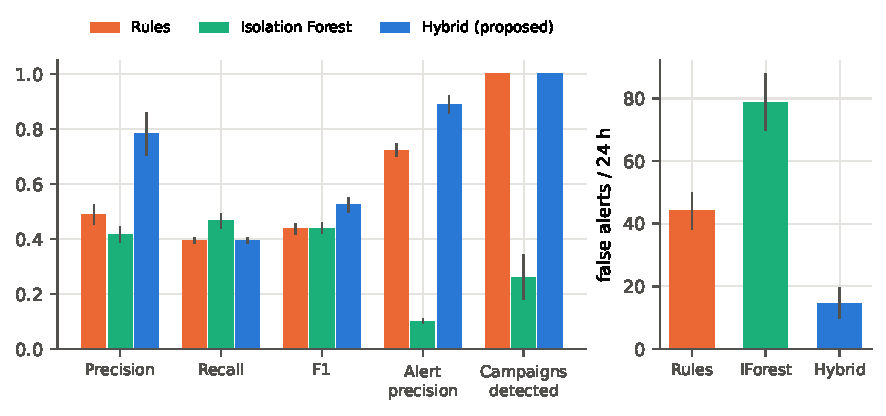
\includegraphics[width=\columnwidth]{figures/e4_detection.pdf}
\caption{E4: detection metrics (left) and false alerts per 24\,h (right).}
\label{fig:e4}
\end{figure}

\subsection*{E5: Correlation and timeline reconstruction}
All correlators receive the same hybrid alerts (Table~\ref{tab:cor}, Fig.~\ref{fig:e5}).

The time-window baseline merges campaigns that overlap in time (homogeneity 0.95, fragmentation 0.81 incidents per campaign). Leader-Follower~\cite{raju2017} produces pure clusters but \emph{fragments} campaigns, at 1.39 (static) and 1.85 (adaptive) incidents per campaign, because its similarity decays with time and multi-hour mining campaigns drift away from their leader.

The entity graph achieves the best ARI (\textbf{0.9996}), V-measure (0.996) and completeness (0.993), with fragmentation 1.19. Reconstruction is the decisive step: alerted events alone cover 34\% of campaign events, while the 2-hop pivot recovers \textbf{100\%} at 0.88 timeline precision. The residual noise is mostly the compromised user's own benign activity inside the window, which an investigator would examine anyway.

\begin{table}[t]
\centering
\caption{E5: correlation and reconstruction (mean over 5 seeds).}
\label{tab:cor}
\footnotesize
\setlength{\tabcolsep}{2.6pt}
\resizebox{\columnwidth}{!}{\begin{tabular}{lcccccc}
\toprule
Correlator & ARI & V & Frag. & Rec.\ (alerts) & Rec.\ (recon.) & Prec. \\
\midrule
Time window & .958 & .972 & 0.81 & .40 & 1.00 & .82 \\
LF static~\cite{raju2017} & .999 & .988 & 1.39 & .33 & .995 & .88 \\
LF adaptive & .998 & .981 & 1.85 & .33 & .990 & .88 \\
\textbf{Entity graph} & \textbf{.9996} & \textbf{.996} & 1.19 & .34 & \textbf{1.00} & \textbf{.88} \\
\bottomrule
\end{tabular}}
\end{table}

\begin{figure}[t]
\centering
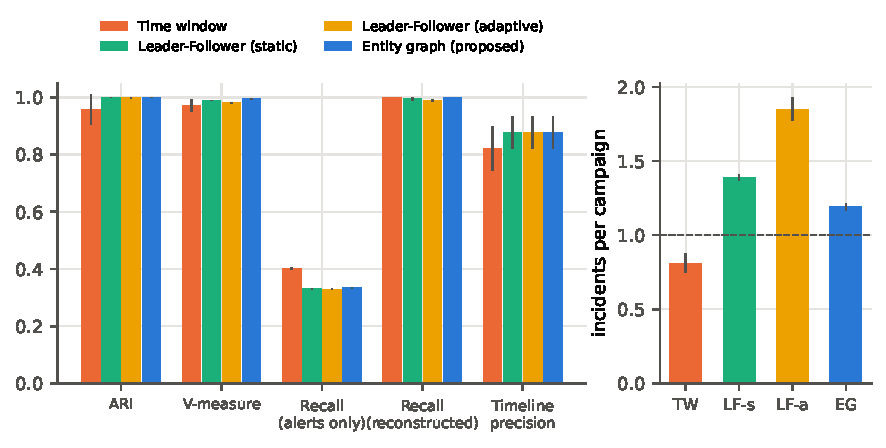
\includegraphics[width=\columnwidth]{figures/e5_correlation.pdf}
\caption{E5: clustering and reconstruction quality (left) and fragmentation (right; 1.0 is ideal).}
\label{fig:e5}
\end{figure}

\paragraph*{Ablation: time normalisation} Treating every timestamp as UTC (``naive'') shifts syslog by the host's zone offset; the mean absolute error is 2.1\,h. Hypervisor events are also shifted by node zone and drift. Fig.~\ref{fig:skew} shows the effect. Detection barely changes (F1 0.520 vs.\ 0.524), since every rule fires within a single source. Reconstruction, however, degrades sharply: overall timeline recall drops to 0.87, recall for SSH lateral movement to \textbf{0.63} and for anti-forensics to 0.72, and cross-source ordering accuracy falls to 0.96. Those are precisely the campaigns that span syslog and API or flow logs. This quantifies the survey's warning about ``distinct time zones'' (Sec.~7.1.2).

\begin{figure}[t]
\centering
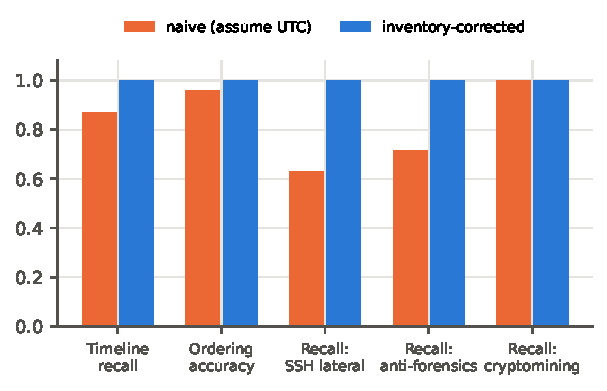
\includegraphics[width=0.92\columnwidth]{figures/e5_time_normalisation.pdf}
\caption{Ablation: naive vs.\ inventory-corrected timestamps.}
\label{fig:skew}
\end{figure}

\subsection*{E6: Evidence isolation}
Over 119 attack incidents, dumping every record in the incident window from shared sources (the common practice) yields about 7,150 records. These contain on average \textbf{51 distinct identifiers of other tenants} and about 5,300 foreign records. The isolated set holds about 2,030 records with zero foreign identifiers, about 200 of them pseudonymised shared records, and it retains \textbf{100\%} of the campaign's records (Fig.~\ref{fig:e6}). This removes the evidence-isolation privacy conflict of Sec.~8.2.4 at no cost to evidence completeness.

\begin{figure}[t]
\centering
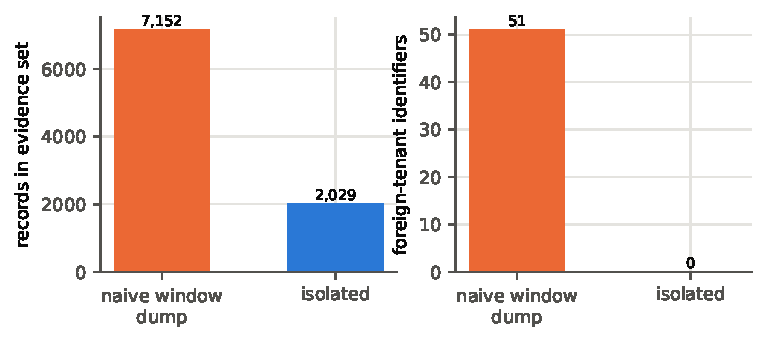
\includegraphics[width=0.85\columnwidth]{figures/e6_isolation.pdf}
\caption{E6: evidence-set size and foreign-tenant identifier leakage per incident.}
\label{fig:e6}
\end{figure}

\subsection*{E7: CSP dependency and acquisition time}
Using Table~14 of the survey, the CDI of an incident is 0.5 for credential exfiltration (storage access logs are held by the CSP), 0.33 for cryptomining (hypervisor), and 0 for the others. All rise to 1.0 if the service owner does not cooperate.

We model acquisition latency with explicit, assumed parameters: owner cooperation is lognormal with median 4\,h (probability 0.8); a legal CSP request is lognormal with median 72\,h and $\sigma{=}1$; sources are requested in parallel. Under this model the status quo has a median EAT of 5--92\,h and a 90th percentile of up to 309\,h (Fig.~\ref{fig:e7}). Forensic readiness on owner-side sources reduces three of the five scenarios to the pipeline's retrieval time, measured in seconds. CSP-held artifacts, however, still dominate exfiltration and mining cases (median about 73\,h). Only a forensics-as-a-service interface from the CSP, the survey's Sec.~8.2.3 recommendation, collapses all scenarios. Because the latencies are assumptions rather than measurements, E7 should be read as a sensitivity illustration of \emph{where} dependency lies, not as a prediction.

\begin{figure}[t]
\centering
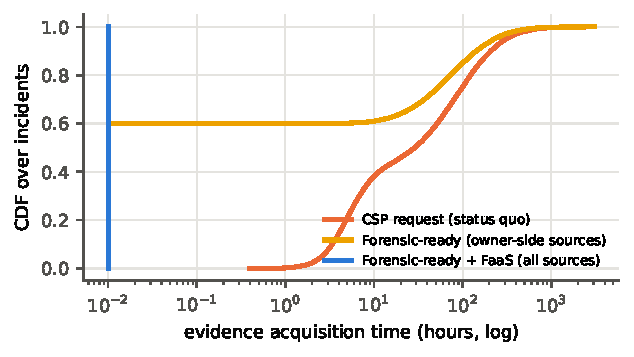
\includegraphics[width=0.92\columnwidth]{figures/e7_acquisition_cdf.pdf}
\caption{E7: modelled evidence-acquisition time over all scenarios.}
\label{fig:e7}
\end{figure}

\subsection*{E8: Scalability}
End-to-end pipeline time grows linearly, from 0.41\,s for 19.5k records (2 tenants, 24\,h) to 5.3\,s for 276k records (16 tenants, 48\,h), a steady \textbf{$\approx$52k records/s} (Fig.~\ref{fig:e8}). Detection and normalisation dominate. Correlation takes under 3\% of the time, and packaging an incident with proofs and a custody ledger takes 4--14\,ms. One core therefore covers about 4.5 billion records per day, so a production deployment would need sharding by tenant for larger regions. The pipeline stages are embarrassingly parallel per tenant.

\begin{figure}[t]
\centering
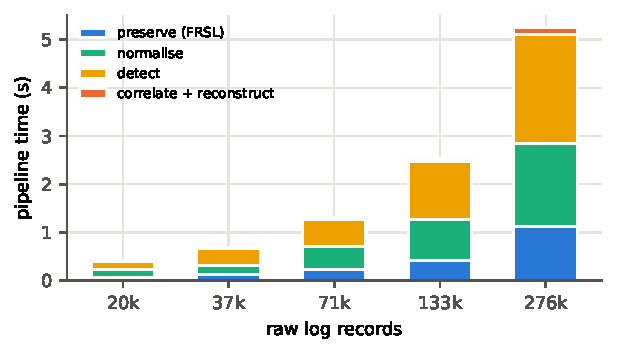
\includegraphics[width=0.92\columnwidth]{figures/e8_scalability.pdf}
\caption{E8: pipeline time per stage against volume.}
\label{fig:e8}
\end{figure}

%=====================================================================
\section{Discussion}
\paragraph*{Mapping back to the survey's guidelines}
\begin{itemize}
\item \emph{Live and remote analysis} (8.2.1): detection runs on streamed logs with an 83\,s MTTD, and needs no physical access.
\item \emph{Log aggregation and correlation} (8.2.2): normalisation and the entity graph raise evidence recall from 34\% to 100\%.
\item \emph{CSP as a forensic contributor} (8.2.3): FRSL makes CSP-held logs ``CSP-proof'', and E7 shows where CSP cooperation still dominates.
\item \emph{Privacy and evidence isolation} (8.2.4): leakage falls from 51 foreign identifiers to 0.
\item \emph{Trusted computing} (8.2.5): tenant-held MAC keys and anchors replace trust in the operator with verification. A TPM-backed key store would strengthen this further.
\end{itemize}

\paragraph*{Limitations and threats to validity}
\begin{enumerate}
\item The data is simulated. Although the formats, confounders and campaign structure are realistic, absolute detection numbers depend on the rule thresholds and the simulator; the \emph{relative} comparisons are the robust finding. Replaying real CloudTrail and VPC Flow datasets is the next step.
\item The detection rules were written with knowledge of the attack classes. Their 100\% campaign recall should not be read as coverage of unknown techniques, which is where the anomaly component matters.
\item FRSL uses a MAC, which requires the verifier to hold $K_T$. Public verifiability would need signatures (for example Ed25519) at a modest cost per epoch.
\item The unsealed-window result shows that seal cadence is a security parameter.
\item The E7 latencies are modelled, not measured.
\end{enumerate}

\section{Conclusion}
We implemented the forensic-investigation guidelines of Manral \textit{et al.}~\cite{manral2019} as \ours{}, an end-to-end monitoring and incident-response framework for multi-tenant clouds, and evaluated it with a reproducible, ground-truth-labelled methodology and a forensic metric suite.

Three findings stand out. First, external anchoring of tenant-keyed Merkle epochs is what defeats a malicious CSP, at a fraction of a blockchain's cost. Second, contextualising rules with behaviour profiles cuts false alerts by two thirds with no loss of campaign coverage. Third, correlation and reconstruction, which depend on correct time normalisation, turn a third of the evidence into all of it.

Future work includes replaying public cloud log datasets, publicly verifiable signatures with TPM-sealed keys, streaming deployment on an ELK/OpenSearch stack, and extending the artifact map to SDN controller and container-orchestrator logs.

\section*{Contribution of Group Members}
Aditya Sharma, Atithi Jaiman and Ashish Singh jointly carried out the survey analysis, the design and implementation of \ours{}, the experimental evaluation, and the writing of this paper.

\begin{thebibliography}{99}
\bibitem{manral2019} B.~Manral, G.~Somani, K.-K.~R. Choo, M.~Conti, and M.~S. Gaur, ``A systematic survey on cloud forensics challenges, solutions, and future directions,'' \emph{ACM Comput. Surv.}, vol.~52, no.~6, art.~124, 2019, doi:10.1145/3361216.
\bibitem{pichan2015} A.~Pichan, M.~Lazarescu, and S.~T. Soh, ``Cloud forensics: Technical challenges, solutions and comparative analysis,'' \emph{Digital Investigation}, vol.~13, pp.~38--57, 2015.
\bibitem{zawoad2016} S.~Zawoad, A.~K. Dutta, and R.~Hasan, ``Towards building forensics enabled cloud through secure logging-as-a-service,'' \emph{IEEE Trans. Dependable Secure Comput.}, vol.~13, no.~2, pp.~148--162, 2016.
\bibitem{ahsan2018} M.~A.~M. Ahsan, A.~W.~A. Wahab, M.~Y.~I. Idris, S.~Khan, E.~Bachura, and K.-K.~R. Choo, ``CLASS: Cloud log assuring soundness and secrecy scheme for cloud forensics,'' \emph{IEEE Trans. Sustain. Comput.}, 2018.
\bibitem{rane2019} S.~Rane and A.~Dixit, ``BlockSLaaS: Blockchain assisted secure logging-as-a-service for cloud forensics,'' in \emph{Proc. Int. Conf. Security and Privacy (ISEA-ISAP)}, Springer, 2019, pp.~77--88.
\bibitem{wang2019} J.~Wang, F.~Peng, H.~Tian, W.~Chen, and J.~Lu, ``Public auditing of log integrity for cloud storage systems via blockchain,'' in \emph{Proc. SPNCE}, Springer, 2019, pp.~378--387.
\bibitem{schneier1999} B.~Schneier and J.~Kelsey, ``Secure audit logs to support computer forensics,'' \emph{ACM Trans. Inf. Syst. Secur.}, vol.~2, no.~2, pp.~159--176, 1999.
\bibitem{crosby2009} S.~A. Crosby and D.~S. Wallach, ``Efficient data structures for tamper-evident logging,'' in \emph{Proc. USENIX Security Symp.}, 2009, pp.~317--334.
\bibitem{trenwith2013} P.~M. Trenwith and H.~S. Venter, ``Digital forensic readiness in the cloud,'' in \emph{Proc. Information Security for South Africa}, IEEE, 2013, pp.~1--5.
\bibitem{marty2011} R.~Marty, ``Cloud application logging for forensics,'' in \emph{Proc. ACM Symp. Applied Computing}, 2011, pp.~178--184.
\bibitem{kebande2015} V.~Kebande and H.~S. Venter, ``A functional architecture for cloud forensic readiness large-scale potential digital evidence analysis,'' in \emph{Proc. European Conf. Cyber Warfare and Security}, 2015, p.~373.
\bibitem{abrahman2016} N.~H. Ab Rahman, W.~B. Glisson, Y.~Yang, and K.-K.~R. Choo, ``Forensic-by-design framework for cyber-physical cloud systems,'' \emph{IEEE Cloud Comput.}, vol.~3, no.~1, pp.~50--59, 2016.
\bibitem{dykstra2013} J.~Dykstra and A.~T. Sherman, ``Design and implementation of FROST: Digital forensic tools for the OpenStack cloud computing platform,'' \emph{Digital Investigation}, vol.~10, pp.~S87--S95, 2013.
\bibitem{alex2017} M.~E. Alex and R.~Kishore, ``Forensics framework for cloud computing,'' \emph{Comput. Electr. Eng.}, vol.~60, pp.~193--205, 2017.
\bibitem{raju2017} B.~K.~S.~P. Raju, N.~B. Gosala, and G.~Geethakumari, ``CLOSER: Applying aggregation for effective event reconstruction of cloud service logs,'' in \emph{Proc. 11th Int. Conf. Ubiquitous Information Management and Communication (IMCOM)}, ACM, 2017, art.~62.
\bibitem{raju2018} B.~K.~S.~P. Kumar Raju and G.~Geethakumari, ``Timeline-based cloud event reconstruction framework for virtual machine artifacts,'' in \emph{Progress in Intelligent Computing Techniques}, Springer, 2018, pp.~31--42.
\bibitem{cohen2011} F.~Cohen, ``Metrics for digital forensics,'' Metricon 5.5, 2011.
\bibitem{liu2008} F.~T. Liu, K.~M. Ting, and Z.-H. Zhou, ``Isolation forest,'' in \emph{Proc. IEEE Int. Conf. Data Mining (ICDM)}, 2008, pp.~413--422.
\bibitem{merkle1987} R.~C. Merkle, ``A digital signature based on a conventional encryption function,'' in \emph{Proc. CRYPTO '87}, Springer, 1987, pp.~369--378.
\bibitem{bloom1970} B.~H. Bloom, ``Space/time trade-offs in hash coding with allowable errors,'' \emph{Commun. ACM}, vol.~13, no.~7, pp.~422--426, 1970.
\bibitem{nist8006} NIST Cloud Computing Forensic Science Working Group, ``NIST cloud computing forensic science challenges,'' NISTIR 8006, 2020.
\bibitem{qi2017} Z.~Qi, C.~Xiang, R.~Ma, J.~Li, H.~Guan, and D.~S.~L. Wei, ``ForenVisor: A tool for acquiring and preserving reliable data in cloud live forensics,'' \emph{IEEE Trans. Cloud Comput.}, vol.~5, no.~3, pp.~443--456, 2017.
\end{thebibliography}

\end{document}
